% Parakeet TDT 1.1B + Chained Linear Adapters — Architecture and gradient flow
% Compile: pdflatex (twice if using references) or latexmk
\documentclass[11pt,a4paper]{article}

\usepackage[margin=1in]{geometry}
\usepackage{amsmath,amssymb,bm}
\usepackage{graphicx}
\usepackage{booktabs}
\usepackage{tikz}
\usetikzlibrary{arrows.meta,positioning,fit,calc,shapes.multipart}
% hyperref last: avoids bookmark / # expansion bugs with tikz and moving arguments
\usepackage{hyperref}
\hypersetup{colorlinks=true,linkcolor=blue,urlcolor=blue,pdfencoding=auto}

\title{Parakeet TDT 1.1B Fine-Tuning:\\
Chained Linear Adapters, NeMo Integration, and Gradient Flow}
\author{(Training setup: \texttt{kaggle\_one\_cell\_nemo\_adapter\_06b\_v2.py})}
\date{}

\begin{document}
\maketitle

\begin{abstract}
This note documents the end-to-end architecture used when fine-tuning NVIDIA Parakeet TDT 1.1B (\texttt{EncDecRNNTBPEModel}) with \emph{chained bottleneck adapters} injected at each Conformer encoder layer. We give tensor shapes, the forward equations for \texttt{ChainedLinearAdapter}, how NeMo routes adapters at semantic locations \texttt{mha} vs.\ \texttt{post}, how residual merging works, and how gradients propagate through the chain state and 42 adapter sites. A one-line registration fix (\texttt{LinearAdapter.register}) is required so NeMo's type check admits the custom module.
\end{abstract}

\tableofcontents
\newpage

%==============================================================================
\section{High-level pipeline}
%==============================================================================

\subsection{Data path (forward)}
Raw audio is converted to log-mel features, then encoded, then decoded with a transducer (RNN-T / TDT) objective.

\begin{center}
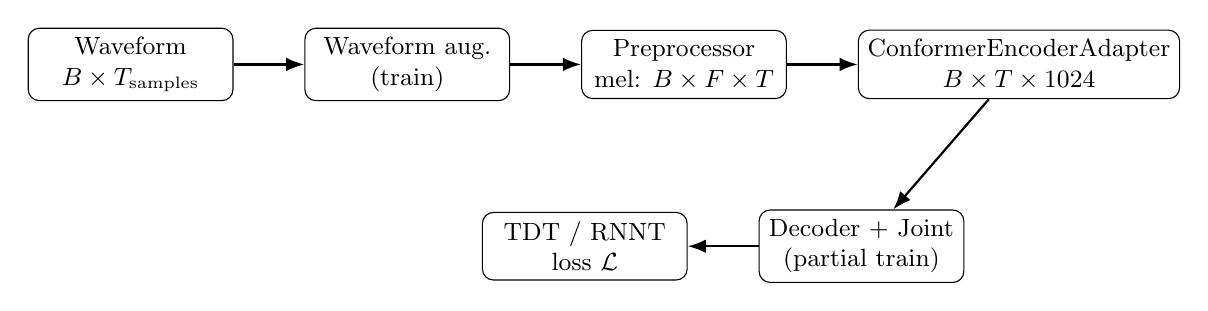
\begin{tikzpicture}[
  node distance=1.1cm and 0.9cm,
  box/.style={rectangle, draw, rounded corners, minimum width=2.6cm, minimum height=0.85cm, align=center, font=\small},
  arrow/.style={-{Latex}, thick}
]
  \node[box] (wav) {Waveform\\$B \times T_\text{samples}$};
  \node[box, right=of wav] (aug) {Waveform aug.\\(train)};
  \node[box, right=of aug] (prep) {Preprocessor\\mel: $B \times F \times T$};
  \node[box, right=of prep] (enc) {ConformerEncoderAdapter\\$B \times T \times 1024$};
  \node[box, below=1.4cm of enc, xshift=-2cm] (dec) {Decoder + Joint\\(partial train)};
  \node[box, left=of dec] (loss) {TDT / RNNT\\loss $\mathcal{L}$};

  \draw[arrow] (wav) -- (aug);
  \draw[arrow] (aug) -- (prep);
  \draw[arrow] (prep) -- (enc);
  \draw[arrow] (enc) -- (dec);
  \draw[arrow] (dec) -- (loss);
\end{tikzpicture}
\end{center}

\noindent
\textbf{Trainable slices} (typical setup): all 42 chained adapters; joint network; decoder embedding and last LSTM layer. Encoder backbone stays frozen in \texttt{eval()}; adapters still run inside frozen Conformer layers because they are separate submodules with \texttt{requires\_grad=True}.

\subsection{Batch and time dimensions}
For a mini-batch, let $B$ be batch size and $T$ the number of encoder frames after subsampling (variable per utterance; padded in batch). Encoder hidden size is $d=1024$. Adapter bottleneck is $r=128$.

%==============================================================================
\section{Conformer layer and where the adapter attaches}
%==============================================================================

Each \texttt{ConformerLayer} applies (schematically): feed-forward $\to$ self-attention $\to$ convolution $\to$ feed-forward, with residuals and layer norms. NeMo's \texttt{AttentionAdapterModuleMixin} calls adapters at two \emph{semantic locations}:

\begin{itemize}
  \item \texttt{loc = mha}: immediately after the main self-attention residual block. The mixin dispatches only if the registered adapter is a \texttt{MultiHeadAttention}-compatible module (not our bottleneck adapter).
  \item \texttt{loc = post}: after the final layer norm, before the layer output. Our \texttt{asr\_children\_adapter} is a bottleneck MLP-style adapter; NeMo runs it here via \texttt{ResidualAddAdapterStrategy}.
\end{itemize}

\noindent
Hence a benign warning \emph{``No adapter compatible with the current module''} can appear once per step at \texttt{mha}: the same adapter name is enabled, but the module type does not match the MHA branch. The bottleneck adapter still runs at \texttt{post} for all 42 layers (verified by 42 forward-hook fires per batch).

\begin{center}
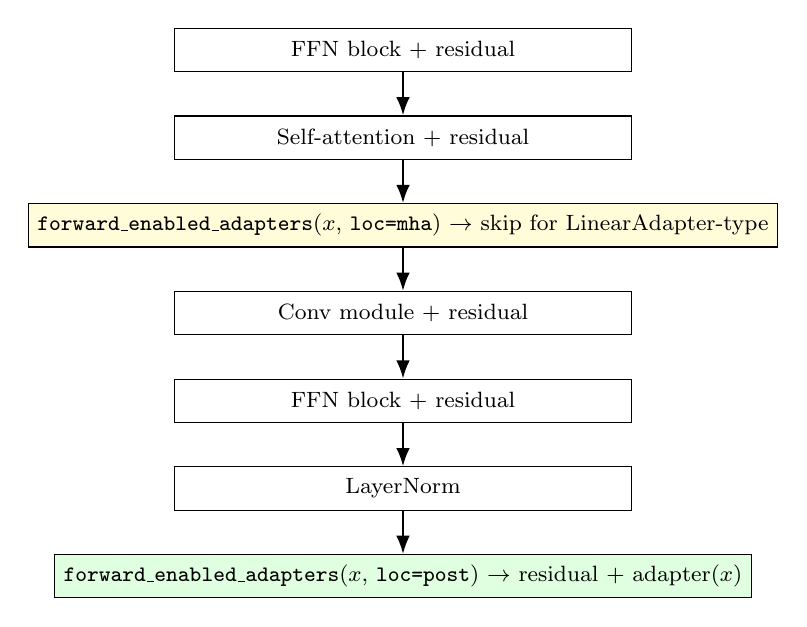
\begin{tikzpicture}[
  node distance=0.55cm,
  box/.style={rectangle, draw, minimum width=5.8cm, minimum height=0.55cm, align=left, font=\footnotesize},
  arrow/.style={-{Latex}, thick}
]
  \node[box] (l1) {FFN block + residual};
  \node[box, below=of l1] (l2) {Self-attention + residual};
  \node[box, below=of l2, fill=yellow!15] (l2a) {\texttt{forward\_enabled\_adapters}($x$, \texttt{loc=mha}) $\to$ skip for LinearAdapter-type};
  \node[box, below=of l2a] (l3) {Conv module + residual};
  \node[box, below=of l3] (l4) {FFN block + residual};
  \node[box, below=of l4] (l5) {LayerNorm};
  \node[box, below=of l5, fill=green!12] (l6) {\texttt{forward\_enabled\_adapters}($x$, \texttt{loc=post}) $\to$ residual + adapter$(x)$};
  \draw[arrow] (l1) -- (l2);
  \draw[arrow] (l2) -- (l2a);
  \draw[arrow] (l2a) -- (l3);
  \draw[arrow] (l3) -- (l4);
  \draw[arrow] (l4) -- (l5);
  \draw[arrow] (l5) -- (l6);
\end{tikzpicture}
\end{center}

%==============================================================================
\section{Chained linear adapter — forward mathematics}
%==============================================================================

\subsection{Shared state across layers}
Let $S$ be an \texttt{AdapterChainState} instance attached to the model. Before each full encoder forward, $S.\texttt{reset}()$ clears:
\[
  S.\texttt{prev\_bottleneck} \gets \varnothing, \qquad S.\texttt{layer\_counter} \gets 0.
\]
During the $\ell$-th adapter forward (in \emph{encoder depth order} after sorting module names), the adapter writes its post-activation bottleneck into $S$.

\subsection{Per-layer map}
Input to the adapter at \texttt{post} is $\bm{x}^{(\ell)} \in \mathbb{R}^{B \times T \times d}$ (same as NeMo's packed tensor $x$). Define learned maps:
\[
  \bm{W}_\text{down}^{(\ell)} \in \mathbb{R}^{r \times d},\quad
  \bm{W}_\text{up}^{(\ell)} \in \mathbb{R}^{d \times r},\quad
  \bm{W}_\text{chain}^{(\ell)} \in \mathbb{R}^{r \times r}\ (\ell>0).
\]

\noindent\textbf{Layer $\ell=0$ (first adapter, no chain projection):}
\begin{align}
  \bm{h}^{(0)} &= \bm{x}^{(0)} (\bm{W}_\text{down}^{(0)})^\top + \bm{b}_\text{down}^{(0)} \quad\in \mathbb{R}^{B\times T\times r}, \\
  \bm{z}^{(0)} &= \sigma\!\left(\bm{h}^{(0)}\right), \quad
  S.\texttt{prev\_bottleneck} \gets \bm{z}^{(0)},\quad S.\texttt{layer\_counter}\mathrel{+}=1, \\
  \bm{u}^{(0)} &= \bm{z}^{(0)} (\bm{W}_\text{up}^{(0)})^\top + \bm{b}_\text{up}^{(0)}, \\
  \hat{\bm{x}}^{(0)} &= \text{LN}(\bm{u}^{(0)}), \quad
  \bm{y}^{(0)} = \text{Dropout}(\hat{\bm{x}}^{(0)}).
\end{align}
Here $\sigma$ is GELU (config). Initialization: $\bm{W}_\text{up}^{(0)}=\bm{0}$, $\bm{b}_\text{up}^{(0)}=\bm{0}$ so the adapter starts as a no-op before training.

\noindent\textbf{Layer $\ell \ge 1$:}
Read $\bm{z}_\text{prev} = S.\texttt{prev\_bottleneck}$ from the \emph{previous} layer's bottleneck (possibly time-resized via nearest-neighbor interpolate if $T$ differs). Then
\begin{align}
  \bm{h}^{(\ell)} &= \bm{x}^{(\ell)} (\bm{W}_\text{down}^{(\ell)})^\top + \bm{b}_\text{down}^{(\ell)}
    + \bm{z}_\text{prev}\, (\bm{W}_\text{chain}^{(\ell)})^\top, \\
  \bm{z}^{(\ell)} &= \sigma\!\left(\bm{h}^{(\ell)}\right), \quad
  \text{update } S \text{ with } \bm{z}^{(\ell)}, \\
  \bm{u}^{(\ell)} &= \bm{z}^{(\ell)} (\bm{W}_\text{up}^{(\ell)})^\top + \bm{b}_\text{up}^{(\ell)}, \\
  \bm{y}^{(\ell)} &= \text{Dropout}\!\left(\text{LN}(\bm{u}^{(\ell)})\right).
\end{align}

\subsection{NeMo residual merge}
NeMo's \texttt{ResidualAddAdapterStrategy} adds the adapter output to the \texttt{post} tensor \emph{before} the adapter call (the residual branch). Schematically, with $\bm{x}^{(\ell)}$ the normalized pre-adapter hidden state at that site:
\[
  \bm{x}^{(\ell)}_\text{out} = \bm{x}^{(\ell)} + \bm{y}^{(\ell)}.
\]
That sum is the identity connection that carries gradient to both branches during backpropagation.

%==============================================================================
\section{Chaining across 42 Conformer layers}
%==============================================================================

\begin{center}
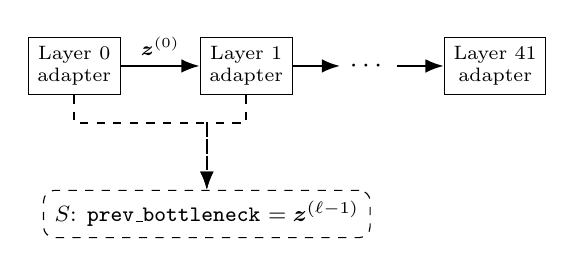
\begin{tikzpicture}[
  node distance=1.0cm,
  lay/.style={rectangle, draw, minimum width=1.1cm, minimum height=0.7cm, font=\scriptsize, align=center},
  chain/.style={-{Latex}, thick},
  state/.style={rectangle, draw, dashed, rounded corners, inner sep=4pt, font=\footnotesize}
]
  \node[lay] (L0) {Layer 0\\adapter};
  \node[lay, right=of L0] (L1) {Layer 1\\adapter};
  \node[right=0.6cm of L1] (dots) {$\cdots$};
  \node[lay, right=0.6cm of dots] (L41) {Layer 41\\adapter};
  \node[state, below=1.2cm of L1, xshift=-0.5cm] (S) {$S$: \texttt{prev\_bottleneck} $=\bm{z}^{(\ell-1)}$};

  \draw[chain] (L0) -- node[above, font=\scriptsize] {$\bm{z}^{(0)}$} (L1);
  \draw[chain] (L1) -- (dots);
  \draw[chain] (dots) -- (L41);
  \draw[chain, dashed] (L0.south) -- ++(0,-0.35) -| (S);
  \draw[chain, dashed] (L1.south) -- ++(0,-0.35) -| (S);
\end{tikzpicture}
\end{center}

\noindent
Important: the chain is in \textbf{bottleneck space} ($r=128$), not in full $d$-dimensional residual space. Each layer still receives its local $\bm{x}^{(\ell)}$ from the frozen Conformer stack; only the low-rank correction is cross-layer coupled.

After a full encoder forward, $S.\texttt{layer\_counter}=42$ (one update per adapter), matching runtime logs.

%==============================================================================
\section{Gradient flow (backward)}
%==============================================================================

\subsection{Autograd view}
PyTorch builds a directed acyclic graph (DAG) of operations. The loss $\mathcal{L}$ depends on all trainable leaves (adapter weights, joint, partial decoder, etc.). For any parameter $\theta$,
\[
  \frac{\partial \mathcal{L}}{\partial \theta} = \sum_{\text{paths}} \frac{\partial \mathcal{L}}{\partial \text{(sink)}} \cdot \frac{\partial \text{(sink)}}{\partial \cdots} \cdots \frac{\partial \cdots}{\partial \theta}.
\]

\subsection{Through the residual}
For merged output $\bm{x}_\text{out} = \bm{x} + \bm{y}(\text{params})$,
\[
  \frac{\partial \mathcal{L}}{\partial \bm{x}} = \frac{\partial \mathcal{L}}{\partial \bm{x}_\text{out}}, \qquad
  \frac{\partial \mathcal{L}}{\partial \text{params}} = \frac{\partial \mathcal{L}}{\partial \bm{x}_\text{out}} \cdot \frac{\partial \bm{y}}{\partial \text{params}}.
\]
Gradients flow into the frozen Conformer trunk as $\partial\mathcal{L}/\partial\bm{x}$ but \emph{no} update is applied to frozen weights ($\texttt{requires\_grad}=\texttt{False}$).

\subsection{Through the bottleneck chain}
The assignment $S.\texttt{prev\_bottleneck} \gets \bm{z}^{(\ell)}$ is a Python side effect, but $\bm{z}^{(\ell)}$ remains a tensor in the graph. When layer $\ell+1$ uses $\bm{z}_\text{prev}$ in
$\bm{h}^{(\ell+1)} = \cdots + \bm{z}_\text{prev} \bm{W}_\text{chain}^\top$,
backpropagation sends gradients to $\bm{W}_\text{chain}^{(\ell+1)}$ and to $\bm{z}_\text{prev}$, hence into layer $\ell$'s GELU, down-projection, and earlier blocks. Thus the chain is not ``truncated'' at the state object: it is standard autograd through shared tensor references.

\subsection{Down-projection gradients early in training}
(Equivalently: why $\partial\mathcal{L}/\partial \bm{W}_{\text{down}}$ can be small at first.) With $\bm{W}_{\text{up}}$ initialized to zero, early in training $\bm{y}\approx\bm{0}$ and most of the signal initially updates $\bm{W}_{\text{up}}$ and upper layers; $\bm{W}_{\text{down}}$ gradients grow once the upper path is non-trivial. Observed logs: \texttt{up} gradients large from step 0; \texttt{down} and \texttt{chain\_proj} ramp up within a few steps.

\subsection{First layer has no chain projection}
The module \texttt{chain\_proj} is absent for the first adapter; $\bm{W}_\text{chain}^{(0)}$ does not exist; logging may show \texttt{chain=nan} when max-abs is taken over a missing parameter --- not a numerical failure.
%==============================================================================
\section{TDT / RNNT loss (schematic)}
%==============================================================================

The model uses a transducer-style loss with token duration targets (TDT). Abstractly,
\[
  \mathcal{L} = -\log \sum_{\text{alignments}} p(\text{alignment} \mid \text{encoder frames}, \text{targets}),
\]
computed with efficient dynamic programming (CUDA kernel). Gradients $\partial\mathcal{L}/\partial \text{logits}$ flow back into the joint network, decoder, and encoder outputs, then into adapters via the residual paths described above.

%==============================================================================
\section{NeMo integration: registering the custom adapter class}
%==============================================================================

\texttt{forward\_single\_enabled\_adapter\_} in \texttt{AttentionAdapterModuleMixin} contains:
\begin{quote}\small
\texttt{if isinstance(adapter\_module, LinearAdapter) and loc == 'post':}\\
\quad run \texttt{adapter\_strategy(x, adapter\_module, ...)}\\
\texttt{else:} \ldots skip with warning.
\end{quote}
\texttt{ChainedLinearAdapter} is implemented as \texttt{nn.Module} + \texttt{AdapterModuleUtil}, not as a subclass of \texttt{LinearAdapter}. Without registration, \texttt{isinstance} fails and every adapter forward is skipped (0 hook fires, no adapter gradients).

\noindent\textbf{Fix:} after constructing adapters,
\begin{verbatim}
LinearAdapter.register(ChainedLinearAdapter)
\end{verbatim}
This ABC ``virtual subclass'' makes \texttt{isinstance(chained, LinearAdapter)} true without inheriting \texttt{LinearAdapter.\_\_init\_\_} (which would be fragile). Then the \texttt{post} branch runs and hooks fire 42 times per forward.

%==============================================================================
\section{Discriminative learning rates (optimizer)}
%==============================================================================

Parameter groups (typical): adapters at $\eta_\text{ad}$; joint at $\eta_\text{joint}$; decoder head at $\eta_\text{dec}$, with $\eta_\text{ad} > \eta_\text{joint} > \eta_\text{dec}$. AdamW updates:
\[
  \theta_{t+1} = \theta_t - \eta \cdot \frac{\hat{\bm{m}}_t}{\sqrt{\hat{\bm{v}}_t} + \epsilon} - \eta \lambda \theta_t
\]
(with decoupled weight decay $\lambda$ on applicable groups).

%==============================================================================
\section{Checklist vs.\ runtime logs}
%==============================================================================

\begin{tabular}{@{}ll@{}}
\toprule
Expected observation & Meaning \\
\midrule
42 adapter hook fires / batch & Each \texttt{post} adapter executed \\
\texttt{layer\_counter} = 42 after encoder & State updated once per adapter \\
\texttt{up} grad $\gg 0$ early & Zero-init upward path receives loss signal \\
\texttt{down} / \texttt{chain} ramp up & Path through bottleneck activates \\
\texttt{chain} nan on layer 0 only & No \texttt{chain\_proj} parameter \\
MHA ``no adapter compatible'' & Expected at \texttt{loc=mha} for bottleneck adapter \\
\bottomrule
\end{tabular}

\vspace{1em}
\noindent
\textbf{Compile:} \texttt{pdflatex parakeet\_tdt\_chained\_adapter\_architecture.tex}

\end{document}
